\section{Experiments}

\subsection{Input data}
To test the correctness of the algorithms we used the MONK's datasets. To use these datasets correctly, we did the following steps:
\begin{itemize}
	\item We preprocessed MONK's datasets with \textit{1-of-k} encoding to convert categorical data to numerical data and we obtained 17 binary input features vectors. This preprocessing is divided between two classes, \textit{Preprocessing} and \textit{LoadDataset}. The former reads, shuffle, and splits the dataset whereas the latter performs the \textit{1-to-k} encoding. 
	\item To view all the networks in vector formulation terms and exploit the \textit{Armadillo} numerical library, we performed batch computation by loading and transposing the entire dataset in a single matrix. The labels were split and saved in another matrix to compute the \textit{MSE} (sez \ref{Loss:Mse}) after the forward phase. To reduce the cost of moving matrices we took advantage of the \textit{move} operator available since C++11. 
	\item Our library can deal with classification and regression tasks exploiting the composition of the \textit{Layer} class.  So we implemented \textit{sigmoid} and \textit{linear} activation functions for the output layer and \textit{hyperbolic tangent} activation function for the hidden layers.
\end{itemize}



To obtain a deterministic behaviour of the algorithms, we used the entire MONKS datasets as the input of the network. We obtained three matrices that had dimensions: 124x18 (Monk 1), 169x17 (Monk 2), and 122x17 (Monk 3). To compare the behaviour of the algorithms, we collected three parameters for every iteration: the error of the network (that is MSE for not regularized network and MSE plus the regularization term for regularized network), the norm of the gradient and the computational time spent on completing the iteration. These parameters were used to make the rate of convergence and the errors with respect to the minima plots shown below. For a better visualization of the plots the y-axis is plotted on a logarithmic scale (except for \S \ref{sec:rate_of_convergence} "Rate of convergence") and an enlargement version of each plots is put on the side. Before showing the plots a table with all the configurations used and the values obtained is shown.

\subsection{Configuration tested}
The notation $f^*$ specifies the optimal value reached by a specific configuration of the problem (that includes the regularization term if it is used). 

\begin{center}
	\small\addtolength{\tabcolsep}{-3pt}
		\centering
		\begin{longtable}{|c|c|c|c|c|c|c|c|c|c|}
			\hline
			\textbf{Task}& \textbf{Optimizer}&\textbf{Model}&\textbf{Iteration} & \textbf{L rate} & \multicolumn{1}{l|}{\textbf{Lambda}} & \textbf{Mom} & \textbf{$f^{*}$}& \textbf{$\Vert \nabla f_{k}\Vert$ }& \textbf{Time(ms)}\\ \hline 
			Monk1 & MDA & M1 & 15000 & 0.9 & 3e-4  & 0.9 & 1.301e-2  & 7.855e-3 & 9161 \\
			Monk1 & MDA & M2 & 15000 & 0.9 & 3e-4  & 0.6 & 2.101e-2 & 6.740e-2 &  2321\\
			Monk1 & NMDA & M1 & 15000 & 0.9 & 3e-4  & 0.9 & 1.143e-2 & 8.343e-3 & 14695 \\
			Monk1 & NMDA & M2 & 15000 & 0.9 & 3e-4  & 0.6 & 1.105e-2 & 3.462e-2 & 5231 \\
			Monk1 & L-BFGS & M1 & 32 & 0.9 & 3e-4  & 0 &  7.939e-2 & 6.324e-6 & 19427  \\
			Monk1 & L-BFGS & M2 & 500 & 0.9 & 3e-4  & 0 &   4.327e-2 & 5.456e-1 & 19362 \\
			Monk1 & PBM & M1 & 2000 & 0.9 & 3e-4  & 0 & 8.796e-2  & 3.869e-5 & 1556359 \\
			Monk1 & PBM & M2 & 54 & 0.9 & 3e-4  & 0 & 8.491e-2 & 1.349e-0 & 100055 \\
			
			Monk2 & MDA & M1 & 15000 & 0.9 & 3e-4  & 0.9 & 1.374e-2 & 1.236e-2 & 20422 \\
			Monk2 & MDA & M2 & 15000 & 0.9 & 3e-4  & 0.6 & 2.264e-2 & 9.747e-2 & 3421 \\
			Monk2 & NMDA & M1 & 15000 & 0.9 & 3e-4  & 0.9 &  1.374e-2 & 1.228e-2 & 18934  \\
			Monk2 & NMDA & M2 & 15000 & 0.9 & 3e-4  & 0.6 & 2.251e-2 & 1.264e-1 & 6098 \\
			Monk2 & L-BFGS & M1 & 381 & 0.9 & 3e-4  & 0 & 6.845e-1 & 9.43e-2 & 27206 \\
			Monk2 & L-BFGS & M2 & 481 & 0.9 & 3e-4  & 0 & 4.542e-2 & 4.294e-1 & 26744 \\
			Monk2 & PBM & M1 & 270 & 0.9 & 3e-4  & 0 & 1.176e-1  & 9.973e-6 & 24036 \\
			Monk2 & PBM & M2 & 2000 & 0.9 & 3e-4  & 0 & 5.958e-6 & 2.647e-4 & 399099 \\
			
			Monk3 & MDA & M1 & 15000 & 0.9 & 3e-4  & 0.9 & 3.458e-2 & 7.675e-2 & 22280 \\
			Monk3 & MDA & M2 & 15000 & 0.9 & 3e-4  & 0.6 & 2.794e-2 & 3.502e-2 & 3458 \\
			Monk3 & NMDA & M1 & 15000 & 0.9 & 3e-4  & 0.9 & 1.587e-2 & 7.145e-3 & 20003 \\
			Monk3 & NMDA & M2 & 15000 & 0.9 & 3e-4  & 0.6 & 2.15e-2 & 8.247e-2 & 3405 \\
			Monk3 & L-BFGS & M1 & 251 & 0.9 & 3e-4  & 0 & 5.608e-2 & 9.905e-2 & 10352 \\
			Monk3 & L-BFGS & M2 & 201 & 0.9 & 3e-4  & 0 & 4.354e-2 & 4.038e-1 & 8314 \\
			Monk3 & PBM & M1 & 1433 & 0.9 & 3e-4  & 0 & 7.423e-2 & 4.994e-5 & 130621 \\
			Monk3 & PBM & M2 & 1434 & 0.9 & 3e-4  & 0 & 7.971e-2 & 4.992e-5 & 129678  \\
			\hline
			\caption{Network configurations with $f^*$.}
			\label{tab:nets_res}
		\end{longtable}

\end{center}

\subsubsection{Methods minima analysis} 

As mentioned in \S\ref{LF:convexity}, the objective function is not convex. For this reason, we try to understand if the methods used were approaching the same optimal value or different ones.
First of all, we analysed the $f^{*}$ value of each configuration to understand at which optimal values the algorithms converge. 

\begin{longtable}{|c|c|c|c|c|c|}
	\hline
	\centering
	\textbf{Optimizer}&\textbf{Iteration} & \textbf{L rate} & \multicolumn{1}{l|}{\textbf{Lambda}} & \textbf{Mom} & \textbf{$f^{*}$} \\ \hline 
	L-BFGS & 50 & - & 3e-4  & 0 & 6.396e-2 \\
	L-BFGS & 50 & - & 5e-4  & 0 & 8.553e-2 \\
	L-BFGS & 50 & - & 7e-4  & 0 & 1.201e-1 \\
	PBM & 400 & - & 5e-4  & 0 & 1.352e-1  \\
	PBM & 400 & - & 7e-4  & 0 & 1.893e-1  \\
	PBM & 400 & - & 3e-4  & 0 & 8.114e-1  \\
	\hline
	\caption{Monk 1 optimizer configuration displayed in increasing order of $f^*$.}
	\label{tab:nets_res_plots_Monk1}
\end{longtable}

As can be seen from table \ref{tab:nets_res_plots_Monk1}, the different configuration of the optimizers MDA and NMDA with 900 iterations converge to the same optimal values. This can be stated because their optimal values differ between 3e-6 and 6e-6. Also for the L-BFGS optimizer with 5e-4 as regularization parameter using 50 iterations and the NMDA with 0.0 as momentum parameter using 900 iterations the optimal values obtained differ of 1e-3.

\begin{longtable}{|c|c|c|c|c|c|}
	\hline
	\centering
	\textbf{Optimizer}&\textbf{Iteration} & \textbf{L rate} & \multicolumn{1}{l|}{\textbf{Lambda}} & \textbf{Mom} & \textbf{$f^{*}$} \\ \hline
	L-BFGS & &  &  & &2 \\ 
	PBM &  & &   &  & \\ 
	\hline
		\caption{Monk 2 optimizer configuration displayed in increasing order of $f^*$.}
	\label{tab:nets_res_plots_Monk2}
\end{longtable}

As can be seen from table \ref{tab:nets_res_plots_Monk2}, the different configurations, with 0.3 and 0.6 as momentum parameter and 0.9 as learning rate, of the optimizers MDA and NMDA with 900 iterations differ of 9e-4 and 5e-4. Also the MDA and NMDA with 0 as momentum parameter obtained the same optimal values. In the end, for the L-BFGS with 5e-4 as regularization parameter and the PBM with 3e-4 as regularization parameter the optimal values obtained differ of 6e-2.  

\begin{longtable}{|c|c|c|c|c|c|}
	\hline
	\centering
	\textbf{Optimizer}&\textbf{Iteration} & \textbf{L rate} & \multicolumn{1}{l|}{\textbf{Lambda}} & \textbf{Mom} & \textbf{$f^{*}$} \\ \hline 
	L-BFGS & 50 & - & 0  & 0 & 8.196e-3 		\\
	PBM & 400 & - & 0  & 0 & 1.231e-2 			\\
	MDA & 900 & 0.9 & 0  & 0.9 & 1.254e-2 	\\
	NMDA & 900 & 0.9 & 0  & 0.9 & 1.254e-2 	\\
	MDA & 900 & 0.9 & 0  & 0.6 & 1.754e-2 	\\
	NMDA & 900 & 0.9 & 0  & 0.6 & 1.754e-2 	\\
	NMDA & 900 & 0.9 & 0  & 0.3 & 1.863e-2 	\\
	MDA & 900 & 0.9 & 0  & 0.3 & 1.864e-2 	\\
	MDA & 900 & 0.9 & 0  & 0 & 1.968e-2 		\\
	NMDA & 900 & 0.9 & 0  & 0 & 1.968e-2 	\\
	L-BFGS & 50 & - & 3e-4  & 0  & 5.781e-2 	\\
	L-BFGS & 50 & - & 7e-4  & 0  & 7.940e-2 	\\
	PBM & 400 & - & 3e-4  & 0 & 7.988e-2 		\\
	L-BFGS & 50 & - & 5e-4  & 0  & 8.555e-2 	\\
	PBM & 400 & - & 5e-4  & 0 & 1.249e-1 		\\
	PBM & 400 & - & 7e-4  & 0 & 1.699e-1 		\\
	\hline
		\caption{Monk 3 optimizer configuration displayed in increasing order of $f^*$.}
	\label{tab:nets_res_plots_Monk3}
\end{longtable}

As can be seen from table \ref{tab:nets_res_plots_Monk3}, the different configuration, with 0.0, 0.3, 0.6 and 0.9 as momentum parameter and 0.9 as learning rate, of the optimizers MDA and NMDA with 900 iterations differ of a maximum of 1e-5. In the end, for the L-BFGS with 7e-4 as regularization parameter and the PBM with 3e-4 as regularization parameter the optimal values obtained differ of 5e-4. 

After further analysis, we observed that the weights initialization influences the  optimal values reached by all the networks after the optimization process.

\subsection{Rate of convergence}
\label{sec:rate_of_convergence}
To compute the rate of convergence for each algorithm, we consider $f^*$ as the optimal value obtained by each of the optimization algorithm (that includes the regularization term if it is used) and $f(x_{k})$ as the optimal value obtained at the iteration $k$ plus the regularization term if it is used. If exists a real positive constant $\gamma$ such that
\begin{equation}
\label{eq:rofFirst}
lim_{k\to \infty}\frac{|f(x_{k+1}) - f^* |}{|f(x_{k}) - f^*|^p} = \gamma > 0,
\end{equation}
we can state that the sequence of values $f(x_{k})$ produced by the algorithm has an order of convergence $p$. In our case, we can derive an alternative faster and rapid procedure to compute it. Considering the equation \ref{eq:rofFirst} we can obtain the following formula: 
\begin{equation}
p = lim_{k\to \infty}\frac{log |f(x_{k+1}) - f^* | - log \gamma}{log|f(x_{k}) - f^*|} \approx lim_{k\to \infty}\frac{log |f(x_{k+1}) - f^* |}{log|f(x_{k}) - f^*|}.
\end{equation}
If $p=1$ the convergence is linear and if $p=2$ the convergence is quadratic. We can observe in figure \ref{CR-Monk2} that L-BFGS reached a superlinear rate of convergence. 
As we expect from the analysis we made, L-BFGS reached a superlinear convergence rate in some epoch. Also for the Momentum Descent Approach, we see that the convergence rate obtained is linear as we expected. Instead, for the Proximal Bundle method we had some convergences rate peaks that we didn't expect. In our opinion, this can be caused by the particular loss shape of Monks dataset.
It's interesting to view that all of these methods, even with a noisy dataset as Monk 3, converge with the same convergence rate as mentioned in the theory. The rate of convergence curves obtained, also with an enlargement for each of them put to the side, are shown below.

\subsubsection{M1 comparison}
\begin{figure}[H]
	\centering
	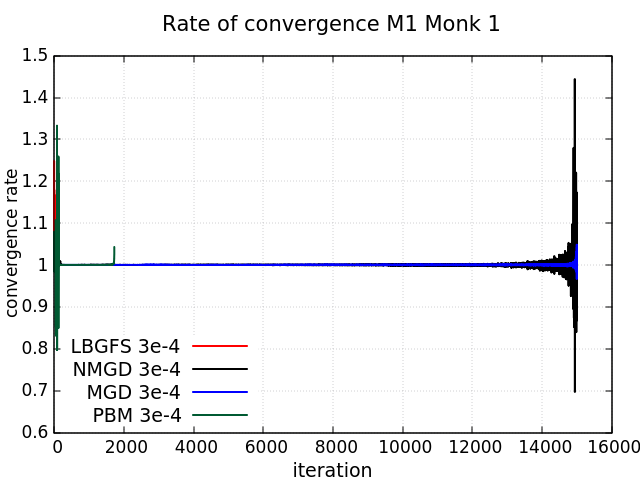
\includegraphics[width=0.6\linewidth]{data/Comparison/Monk1/Monk1_M1_CR_standard.png}
	\caption{M1 converge rate comparison Monk 1 of configurations defined in table \ref{tab:nets_comp}.}
	\label{fig:CR-M1-Monk1-Standard}
\end{figure}

\begin{figure}[H]
	\centering
	\begin{minipage}[t]{0.525\linewidth}		
		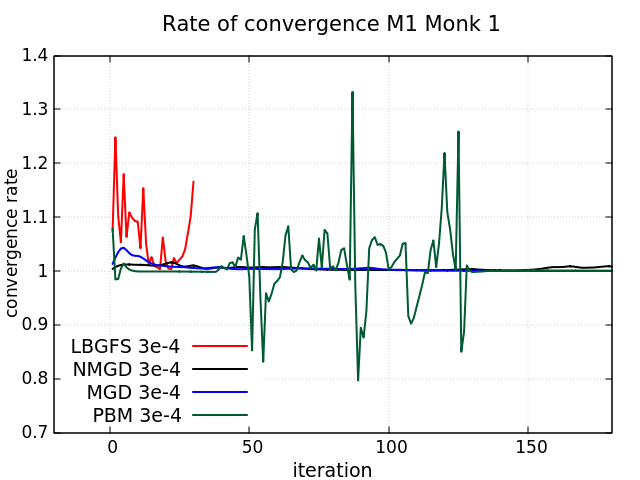
\includegraphics[width=\linewidth]{data/Comparison/Monk1/Monk1_M1_CR_zoomLeft.png}
		\subcaption{Left zoom}
	\end{minipage}%
	\begin{minipage}[t]{0.525\linewidth}
		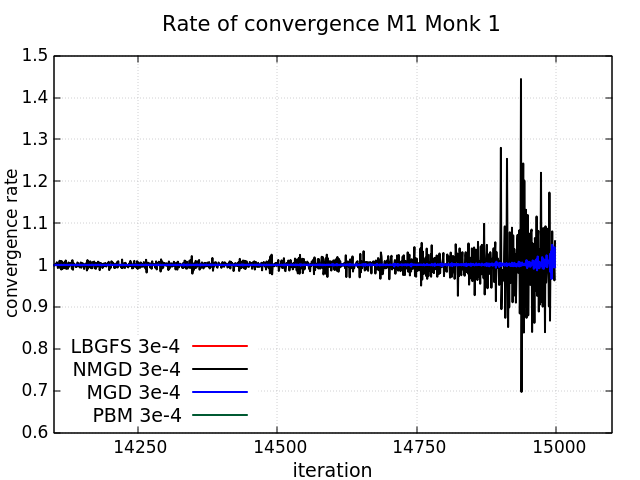
\includegraphics[width=\linewidth]{data/Comparison/Monk1/Monk1_M1_CR_zoomRight.png}
		\subcaption{Right zoom}
	\end{minipage}
	\caption{M1 converge rate comparison Monk 1 of configurations defined in table \ref{tab:nets_comp}.}
	\label{fig:CR-M1-Monk1-Zoom}
\end{figure}

\begin{figure}[H]
	\centering
	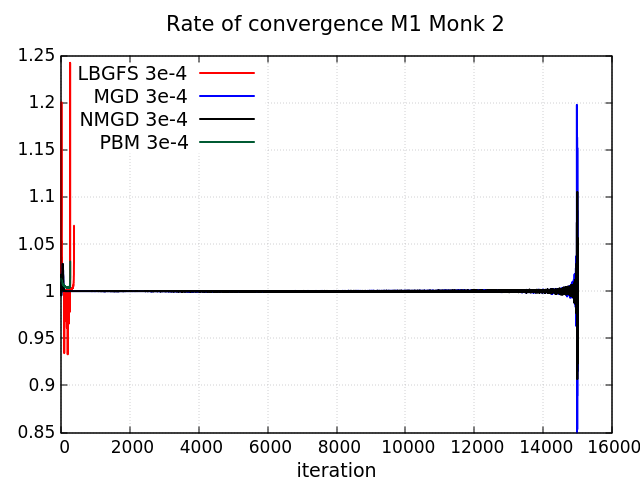
\includegraphics[width=0.6\linewidth]{data/Comparison/Monk2/Monk2_M1_CR_standard.png}
	\caption{M1 converge rate comparison Monk 2 of configurations defined in table \ref{tab:nets_comp}.}
	\label{fig:CR-M1-Monk2-Standard}
\end{figure}

\begin{figure}[H]
	\centering
	\begin{minipage}[t]{0.525\linewidth}		
		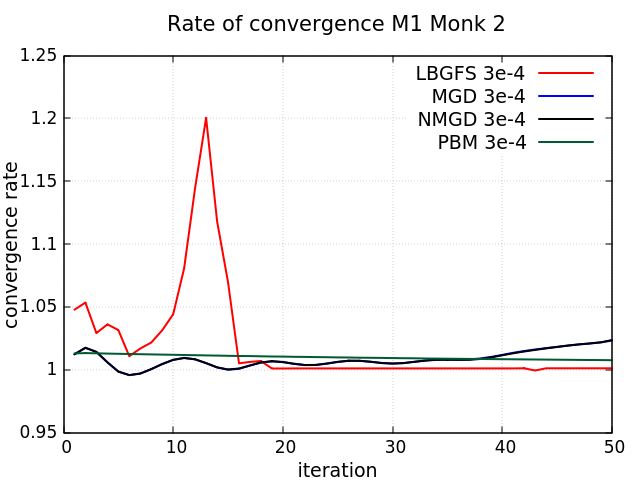
\includegraphics[width=\linewidth]{data/Comparison/Monk2/Monk2_M1_CR_zoomLeft.png}
		\subcaption{Left zoom}
	\end{minipage}%
	\begin{minipage}[t]{0.525\linewidth}
		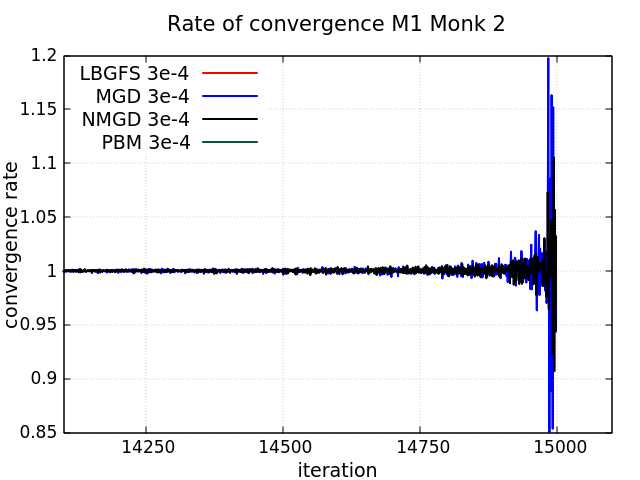
\includegraphics[width=\linewidth]{data/Comparison/Monk2/Monk2_M1_CR_zoomRight.png}
		\subcaption{Right zoom}
	\end{minipage}
	\caption{M1 converge rate comparison Monk 2 of configurations defined in table \ref{tab:nets_comp}.}
	\label{fig:CR-M1-Monk2-Zoom}
\end{figure}

\begin{figure}[H]
	\centering
	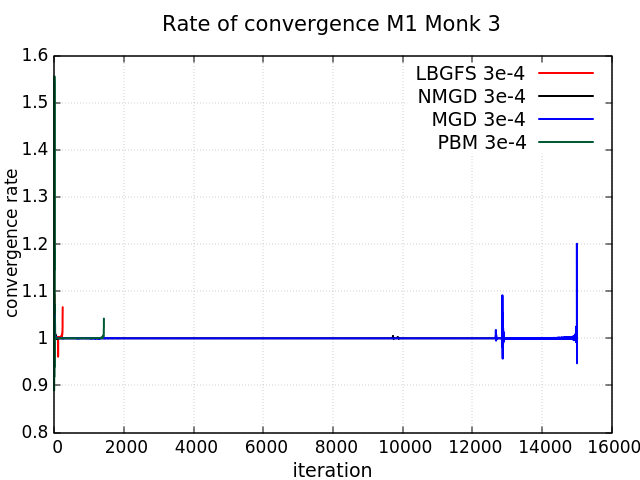
\includegraphics[width=0.6\linewidth]{data/Comparison/Monk3/Monk3_M1_CR_standard.png}
	\caption{M1 converge rate comparison Monk 3 of configurations defined in table \ref{tab:nets_comp}.}
	\label{fig:CR-M1-Monk3-Standard}
\end{figure}

\begin{figure}[H]
	\centering
	\begin{minipage}[t]{0.525\linewidth}		
		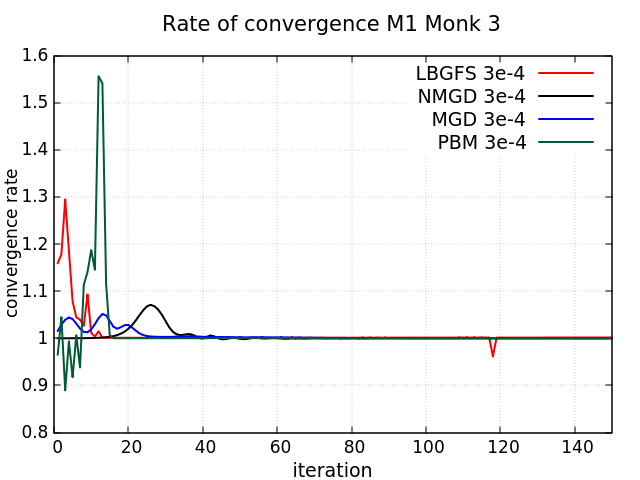
\includegraphics[width=\linewidth]{data/Comparison/Monk3/Monk3_M1_CR_zoomLeft.png}
		\subcaption{Left zoom}
	\end{minipage}%
	\begin{minipage}[t]{0.525\linewidth}
		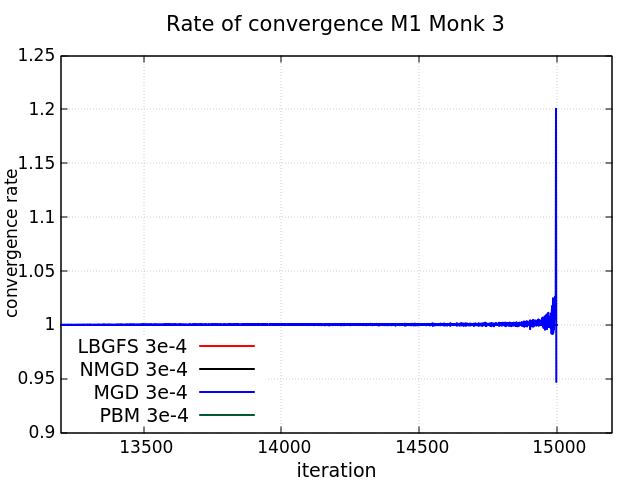
\includegraphics[width=\linewidth]{data/Comparison/Monk3/Monk3_M1_CR_zoomRight.png}
		\subcaption{Right zoom}
	\end{minipage}
	\caption{M1 converge rate comparison Monk 3 of configurations defined in table \ref{tab:nets_comp}.}
	\label{fig:CR-M1-Monk3-Zoom}
\end{figure}

\subsubsection{M2 comparison}
\begin{figure}[H]
	\centering
	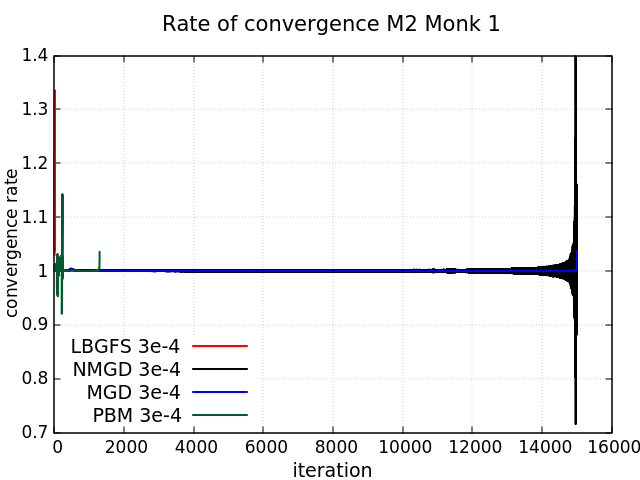
\includegraphics[width=0.6\linewidth]{data/Comparison/Monk1/Monk1_M2_CR_standard.png}
	\caption{M2 converge rate comparison Monk 1 of configurations defined in table \ref{tab:nets_comp}.}
	\label{fig:CR-M2-Monk1-Standard}
\end{figure}

\begin{figure}[H]
	\centering
	\begin{minipage}[t]{0.525\linewidth}		
		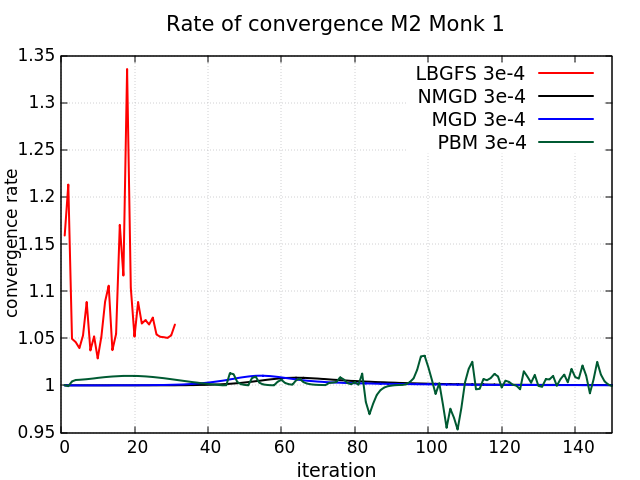
\includegraphics[width=\linewidth]{data/Comparison/Monk1/Monk1_M2_CR_zoomLeft.png}
		\subcaption{Left zoom}
	\end{minipage}%
	\begin{minipage}[t]{0.525\linewidth}
		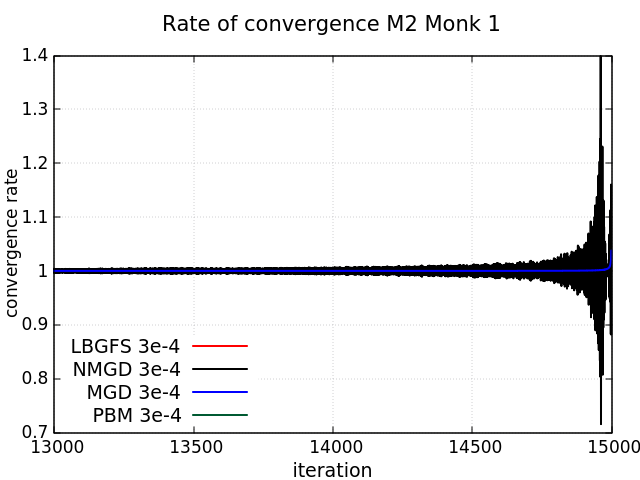
\includegraphics[width=\linewidth]{data/Comparison/Monk1/Monk1_M2_CR_zoomRight.png}
		\subcaption{Right zoom}
	\end{minipage}
	\caption{M2 converge rate comparison Monk 1 of configurations defined in table \ref{tab:nets_comp}.}
	\label{fig:CR-M2-Monk1-Zoom}
\end{figure}

\begin{figure}[H]
	\centering
	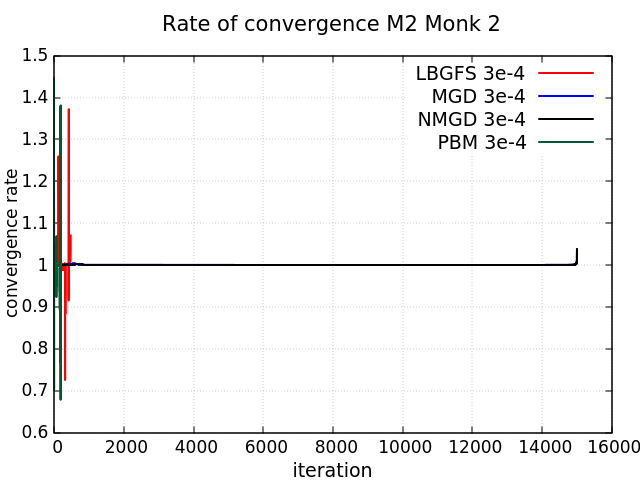
\includegraphics[width=0.6\linewidth]{data/Comparison/Monk2/Monk2_M2_CR_standard.png}
	\caption{M2 converge rate comparison Monk 2 of configurations defined in table \ref{tab:nets_comp}.}
	\label{fig:CR-M2-Monk2-Standard}
\end{figure}

\begin{figure}[H]
	\centering
	\begin{minipage}[t]{0.525\linewidth}		
		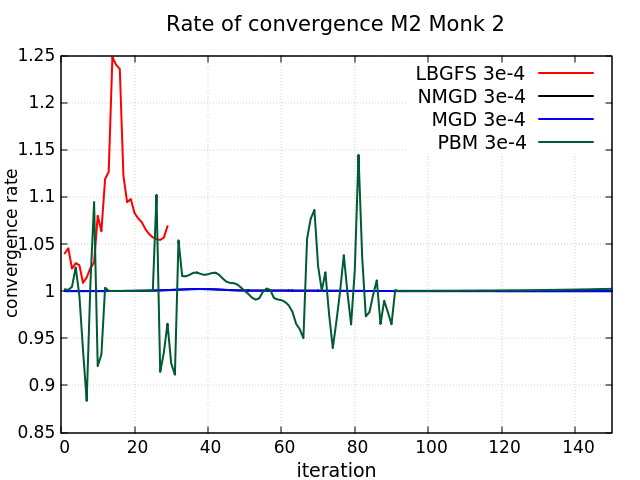
\includegraphics[width=\linewidth]{data/Comparison/Monk2/Monk2_M2_CR_zoomLeft.png}
		\subcaption{Left zoom}
	\end{minipage}%
	\begin{minipage}[t]{0.525\linewidth}
		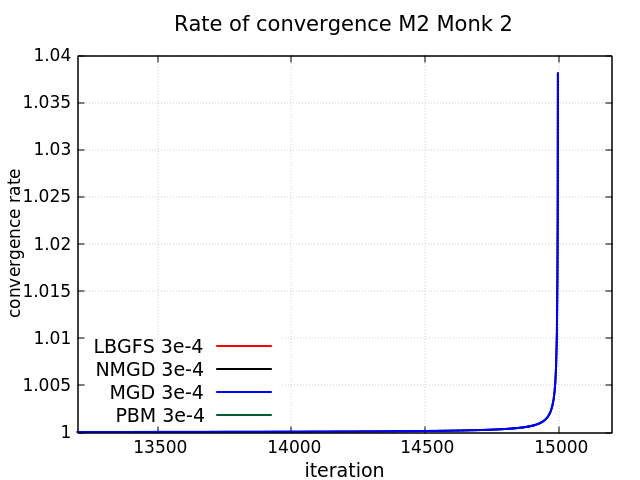
\includegraphics[width=\linewidth]{data/Comparison/Monk2/Monk2_M2_CR_zoomRight.png}
		\subcaption{Right zoom}
	\end{minipage}
	\caption{M2 converge rate comparison Monk 2 of configurations defined in table \ref{tab:nets_comp}.}
	\label{fig:CR-M2-Monk2-Zoom}
\end{figure}

\begin{figure}[H]
	\centering
	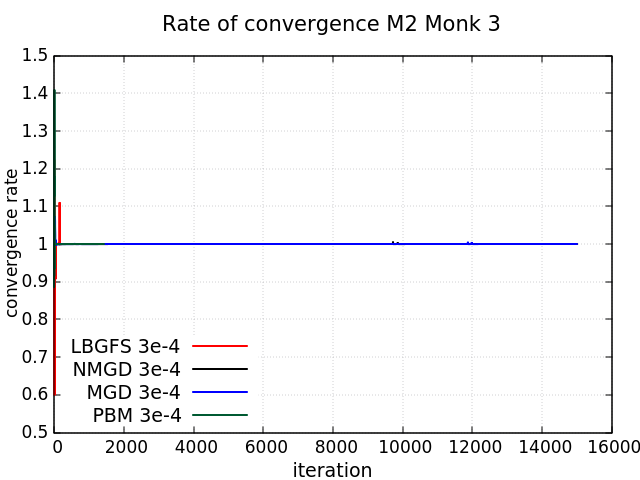
\includegraphics[width=0.6\linewidth]{data/Comparison/Monk3/Monk3_M2_CR_standard.png}
	\caption{M2 converge rate comparison Monk 3 of configurations defined in table \ref{tab:nets_comp}.}
	\label{fig:CR-M2-Monk3-Standard}
\end{figure}

\begin{figure}[H]
	\centering
	\begin{minipage}[t]{0.525\linewidth}		
		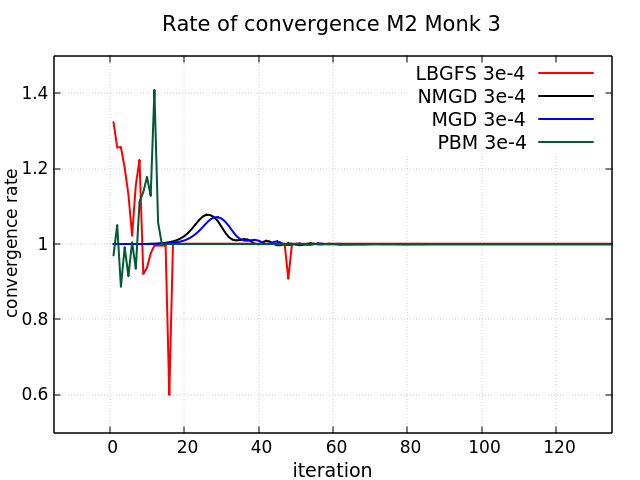
\includegraphics[width=\linewidth]{data/Comparison/Monk3/Monk3_M2_CR_zoomLeft.png}
		\subcaption{Left zoom}
	\end{minipage}%
	\begin{minipage}[t]{0.525\linewidth}
		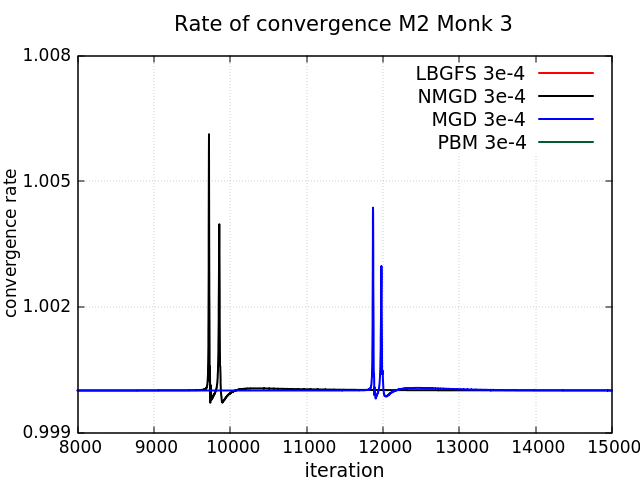
\includegraphics[width=\linewidth]{data/Comparison/Monk3/Monk3_M2_CR_zoomRight.png}
		\subcaption{Right zoom}
	\end{minipage}
	\caption{M2 converge rate comparison Monk 3 of configurations defined in table \ref{tab:nets_comp}.}
	\label{fig:CR-M2-Monk3-Zoom}
\end{figure}


\subsection{Errors with respect to the minima}
\label{sec:minimum_error}
The error with respect to the minimum for each iteration is obtained by the following formula: $ f(x_k) - f^*$ where  $f(x_{k})$ is the MSE obtained at the iteration $k$ plus the  regularization term if it is used and $f^*$ is the optimal value reached by the specific configuration of the problem (that includes the regularization term if it is used). The plots of the error with respect to the minimum value obtained from the configurations in the table \ref{tab:nets_comp} are shown below, also an enlargement for each of them is put to the side.

An important thing to notice is that $f^*$ might not be 0 because it depends on the function that we minimize (that is only the MSE for not regularized network and the MSE plus the regularization term for regularized network). This function could be not convex and due to this fact, it could have multiple local minima in which we could stop. For this reason, to understand if an algorithm has converged to a local minimum, that cannot reach an error equal to zero, but it is still a minimum, the norm of the gradient has to be checked to understand how far from the stationary point (and how far from the end of convergence) we are. \texttt{This can be seen in Monk 3 with L-BFGS optimizer without regularization in which the $f^*$ obtained is 8.198e-3 but the norm of the gradient is 1.9e-6, so the algorithm has converged near a local minimum.}

\subsubsection{M1 comparison}

\begin{figure}[H]
	\centering
	\begin{minipage}[t]{0.5\linewidth}
		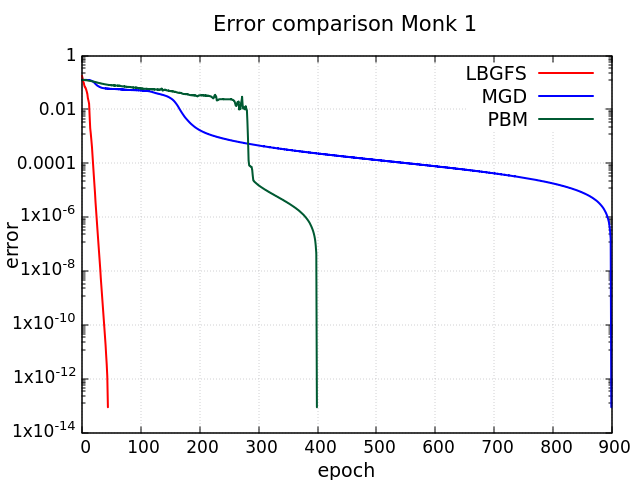
\includegraphics[width=\linewidth]{data/Comparison/Monk1/Monk1_R_Comparison_log_standard.png}
		\subcaption{Original}
	\end{minipage}%
	\begin{minipage}[t]{0.5\linewidth}
		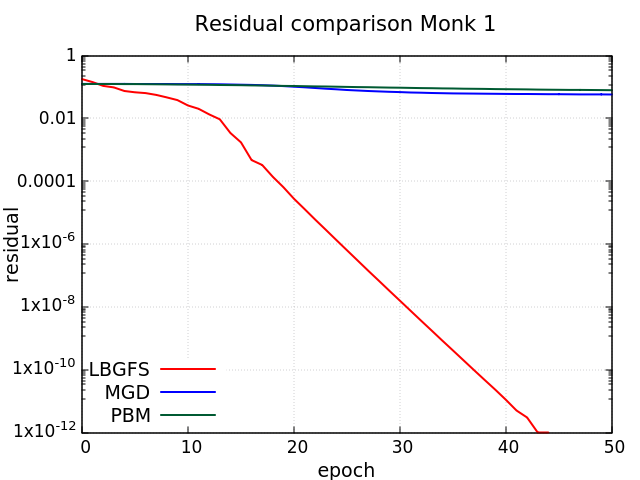
\includegraphics[width=\linewidth]{data/Comparison/Monk1/Monk1_R_Comparison_log_zoom.png}
		\subcaption{Zoom}
	\end{minipage}
	\caption{Errors with respect to the minimum comparison Monk 1 of configurations defined in table \ref{tab:nets_comp}}
	\label{R-Monk1}
\end{figure}


\subsubsection{M2 comparison}


\begin{figure}[H]
	\centering
	\begin{minipage}[t]{0.6\linewidth}
		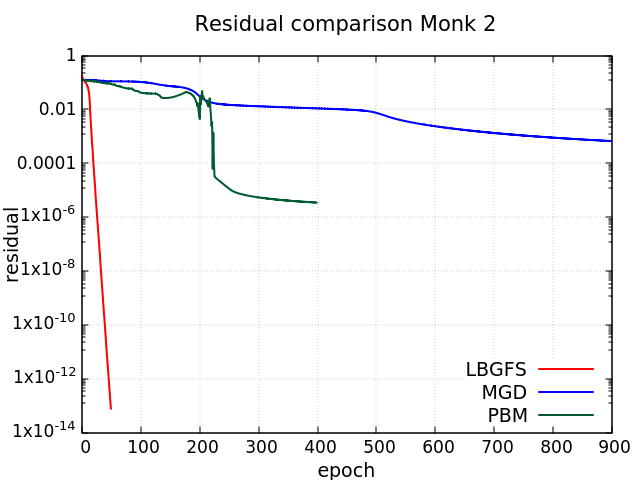
\includegraphics[width=\linewidth]{data/Comparison/Monk2/Monk2_R_Comparison_log_standard.png}
		\subcaption{Original}
	\end{minipage}%
	\begin{minipage}[t]{0.6\linewidth}
		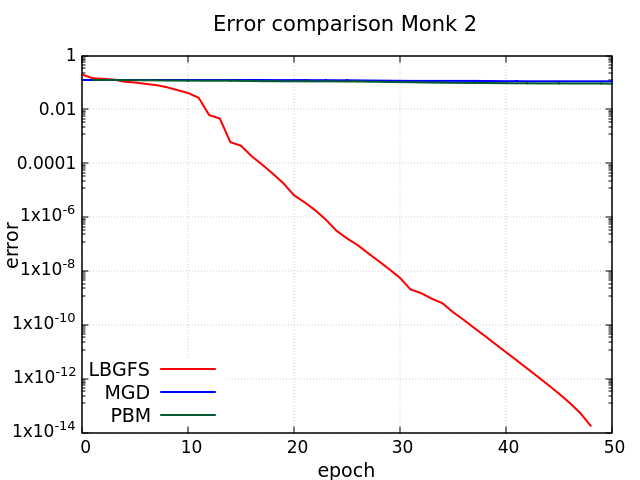
\includegraphics[width=\linewidth]{data/Comparison/Monk2/Monk2_R_Comparison_log_zoom.png}
		\subcaption{Zoom}
	\end{minipage}
	\caption{Errors with respect to the minimum comparison Monk 2 of configurations defined in table \ref{tab:nets_comp}}
	\label{R-Monk2}
\end{figure}
\begin{figure}[H]
	\centering
	\begin{minipage}[t]{0.5\linewidth}
		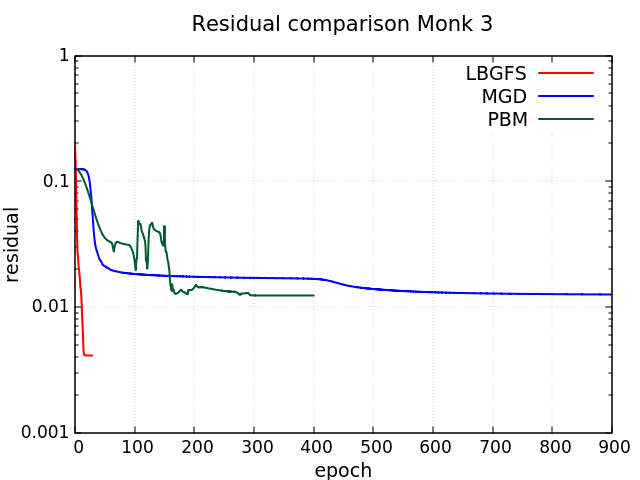
\includegraphics[width=\linewidth]{data/Comparison/Monk3/Monk3_R_Comparison_log_standard.png}
		\subcaption{Original}
	\end{minipage}%
	\begin{minipage}[t]{0.5\linewidth}
		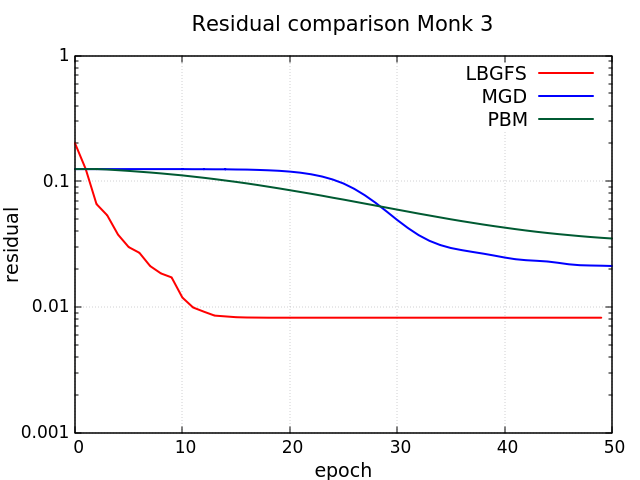
\includegraphics[width=\linewidth]{data/Comparison/Monk3/Monk3_R_Comparison_log_zoom.png}
		\subcaption{Zoom}
	\end{minipage}
	\caption{Errors with respect to the minimum comparison Monk 3 of configurations defined in table \ref{tab:nets_comp}}
	\label{R-Monk3}
\end{figure}